\documentclass{article}

\usepackage[final]{neurips_2024}

\usepackage[utf8]{inputenc}
\usepackage[T1]{fontenc}
\usepackage{hyperref}
\usepackage{url}
\usepackage{booktabs}
\usepackage{amsfonts}
\usepackage{nicefrac}
\usepackage{microtype}
\usepackage{xcolor}
\usepackage{graphicx}

\graphicspath{{../figures/}}

\title{DSC 291 Trustworthy ML Group 7 Final Project Report}

\author{%
  Zach Liu\\
  \texttt{zaliu@ucsd.edu} \\
  \And
  April Chen\\
  \texttt{q8chen@ucsd.edu} \\
  \And
  Inno Li\\
  \texttt{yil167@ucsd.edu} \\
  \And
  Xuanwen Hua\\
  \texttt{x2hua@ucsd.edu} \\
  \And
  Nanami Huang\\
  \texttt{n8huang@ucsd.edu} \\
}

\begin{document}

\maketitle

\section{Introduction}

Large language models are now deployed behind chat assistants, coding copilots, search systems, and tool-using agents. Once a model can take actions on behalf of a user, refusal behavior becomes a security property rather than a nicety. A jailbreak is an adversarial input crafted to bypass a model's safety alignment and elicit content it was trained to refuse.

Jailbreak robustness is difficult to compare across papers because reported attack success rates (ASRs) depend on many hidden choices: target model snapshot, attack prompt set, generation settings, and especially the judge used to label a response as successful or refused. JailbreakBench \cite{chao2024jailbreakbench} addresses this by releasing a fixed behavior dataset, versioned PAIR and GCG attack artifacts, a judge specification, and a public leaderboard.

We reproduce a scoped slice of JailbreakBench on one open-weight local model, \texttt{lmsys/vicuna-13b-v1.5}, and one closed-source API model, \texttt{gpt-4o-mini}. We use a stratified 30-behavior harmful subset with 30 matched benign behaviors, load the public PAIR and GCG artifacts for Vicuna, and score responses with Llama-Guard-2 as our primary judge. We then extend the reproduction with a dictionary-filter defense, benign over-refusal checks, four-judge sensitivity analysis, and repeated private API judge calls across times of day.

Our headline result is that the Vicuna reproduction matches the paper's PAIR ASR closely and reproduces GCG directionally, while GPT-4o-mini is much less vulnerable to the same transferred Vicuna-targeted artifacts. The strongest methodological result is judge sensitivity: the same saved responses can move by up to 24 percentage points depending only on the judge.

\section{Background and Related Work}

\textbf{Jailbreak attacks.} PAIR \cite{chao2023pair} is a black-box attack that uses an attacker LLM to iteratively refine a prompt against a target model. Its prompts are fluent and human-readable, closer to social engineering than token-level optimization. GCG \cite{zou2023gcg} is a white-box, gradient-based attack that optimizes an adversarial suffix appended to a harmful request. GCG prompts often look like unnatural strings of tokens, and this form strongly affects both transferability and defenses.

\textbf{Defenses.} Prior work such as SmoothLLM \cite{robey2024smoothllm} perturbs prompts and aggregates responses, exploiting the brittleness of GCG-style suffixes. Our defense is much simpler: \texttt{dictionary\_filter}, a prompt preprocessor that removes non-dictionary tokens before generation. It is not a complete defense, but it is a useful baseline for testing whether suffix-heavy attacks are easier to disrupt than natural-language attacks.

\textbf{Evaluation and judging.} Deciding whether a response constitutes a successful jailbreak requires a judge. JailbreakBench's reference pipeline uses a Llama-3-70B-based judge, while Llama Guard \cite{inan2023llamaguard} is a dedicated input-output safety classifier often reused as an automated jailbreak judge. Our extension focuses on this measurement layer: if two judges disagree on the same response, ASR is partly a property of the evaluator, not just the target model.

\section{Approach}

Our goal was not to rebuild the entire JailbreakBench leaderboard. Instead, we reproduced a focused subset, verified the paper's core attack-method ranking on Vicuna, and then tested how robust the measured number is to defense and judge choices.

The pipeline is:
\begin{enumerate}
  \item Sample a 30-behavior harmful subset from JBB-Behaviors with seed 291, plus 30 matched benign behaviors.
  \item Load public PAIR and GCG jailbreak artifacts released for \texttt{vicuna-13b-v1.5}.
  \item Generate responses from Vicuna locally and GPT-4o-mini through the OpenAI API.
  \item Score saved responses with Llama-Guard-2 and additional sensitivity judges.
  \item Aggregate attack success rate and benign refusal metrics.
  \item Extend with a dictionary-filter defense and repeated private API judge calls.
\end{enumerate}

We wrapped this workflow in the repository under \texttt{src/jbb\_repro/}, with configuration files, scripts, a Colab driver notebook, and unit tests. Some sampled behaviors do not have both PAIR and GCG artifacts, so final method counts are 29 for GCG and 25 for PAIR rather than exactly 30.

\section{Experiments}

\begin{table}[h]
\centering
\begin{tabular}{ll}
\toprule
Item & Setting \\
\midrule
Harmful behaviors & 30 stratified samples, seed 291 \\
Benign behaviors & 30 matched samples, seed 291 \\
Open-weight target & \texttt{lmsys/vicuna-13b-v1.5} on A100 80GB \\
Closed-source target & \texttt{gpt-4o-mini} via API \\
Attacks & PAIR and GCG artifacts for Vicuna \\
Primary judge & Llama-Guard-2-8B \\
Sensitivity judges & GPT-4o-mini judge, Llama-Guard-3-8B, heuristic \\
Defense & \texttt{dictionary\_filter} on Vicuna \\
\bottomrule
\end{tabular}
\caption{Experimental setup.}
\label{tab:experiment_setup}
\end{table}

Our main metric is attack success rate:
\[
\text{ASR} = \frac{\# \text{successful jailbreaks}}{\# \text{tested harmful behaviors}}.
\]
For benign behaviors, we report refusal rate when using refusal judges and unsafe rate when using Llama Guard. Llama Guard is not a refusal detector, so its benign numbers are auxiliary safety signals rather than over-refusal metrics.

\section{Key Results and Analysis}

\subsection{Vicuna Reproduction}

\begin{table}[h]
\centering
\begin{tabular}{lccc}
\toprule
Attack & Paper Vicuna ASR & Our ASR (LG2) & n \\
\midrule
PAIR & 0.690 & 0.680 & 25 \\
GCG & 0.800 & 0.862 & 29 \\
\bottomrule
\end{tabular}
\caption{Vicuna reproduction results compared with the original JailbreakBench report.}
\label{tab:vicuna_results}
\end{table}

\begin{figure}[h]
\centering
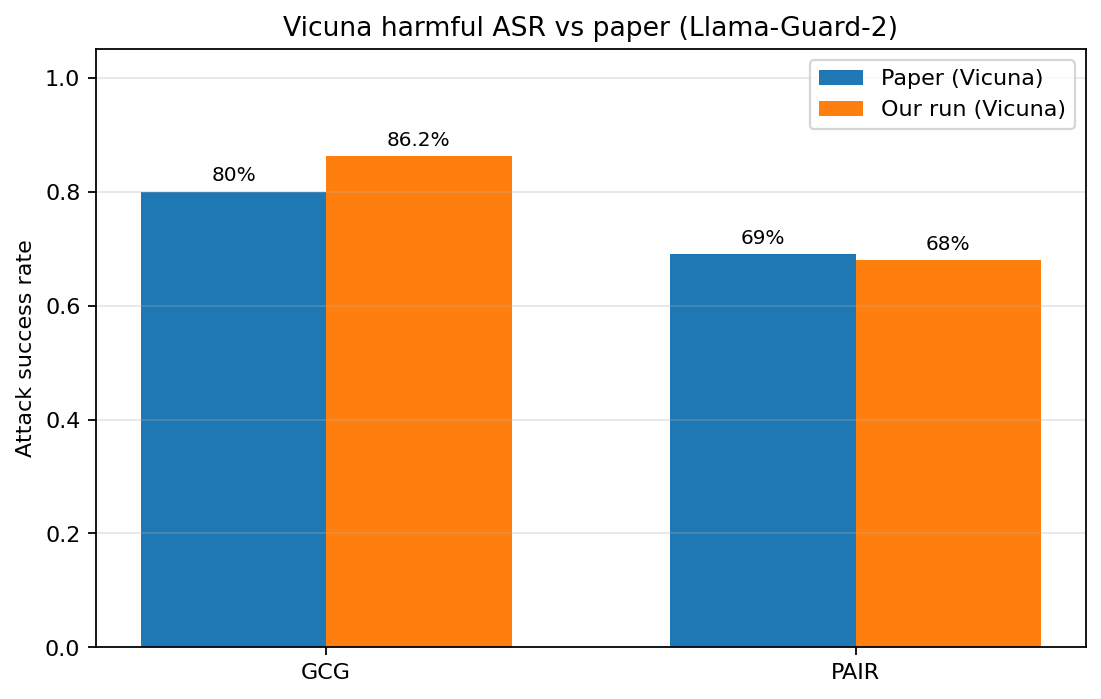
\includegraphics[width=0.75\linewidth]{vicuna_asr_vs_paper_llamaguard.png}
\caption{Our reproduced Vicuna ASR next to the paper's reported values.}
\label{fig:vicuna_paper}
\end{figure}

PAIR reproduces almost exactly: our Llama-Guard-2 ASR is 0.680 compared with the paper's 0.690. GCG is directionally aligned but higher, 0.862 compared with 0.800. The gap is plausible given the smaller subset, different judge, and artifact coverage. The core paper-level ordering remains: Vicuna is highly vulnerable to both methods, and especially to GCG.

\subsection{Open vs. Closed Model}

\begin{table}[h]
\centering
\begin{tabular}{llcc}
\toprule
Model & Method & n & ASR (LG2) \\
\midrule
Vicuna-13B & GCG & 29 & 0.862 \\
Vicuna-13B & PAIR & 25 & 0.680 \\
GPT-4o-mini & GCG & 29 & 0.103 \\
GPT-4o-mini & PAIR & 25 & 0.240 \\
\bottomrule
\end{tabular}
\caption{Harmful ASR under the primary Llama-Guard-2 judge.}
\label{tab:open_closed}
\end{table}

\begin{figure}[h]
\centering
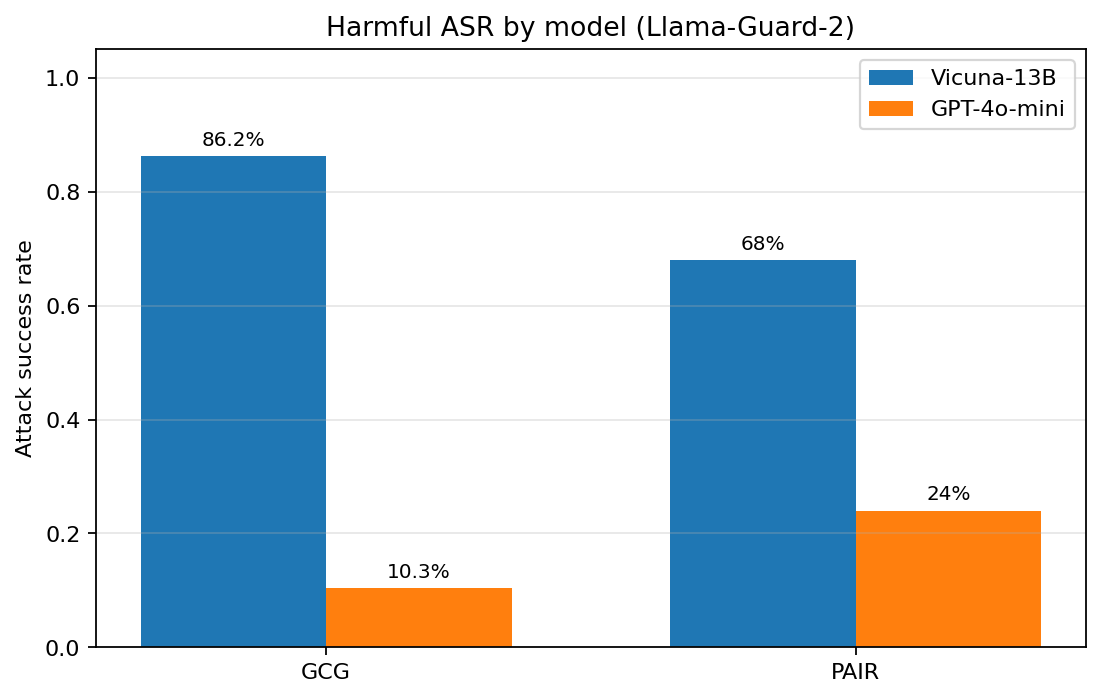
\includegraphics[width=0.75\linewidth]{harmful_asr_by_model_llamaguard.png}
\caption{Harmful ASR by model under Llama-Guard-2.}
\label{fig:harmful_by_model}
\end{figure}

GPT-4o-mini is much less vulnerable to the same transferred prompts. Under Llama-Guard-2, GCG falls from 0.862 on Vicuna to 0.103 on GPT-4o-mini, and PAIR falls from 0.680 to 0.240. These results should be read as transfer results, not a complete robustness claim about GPT-4o-mini, because the artifacts were optimized for Vicuna rather than for the API model.

\subsection{Benign Behaviors}

\begin{table}[h]
\centering
\begin{tabular}{lccccc}
\toprule
Model & n & Heuristic refusal & GPT refusal & LG2 unsafe & LG3 unsafe \\
\midrule
Vicuna-13B & 30 & 0.000 & 0.033 & 0.100 & 0.000 \\
\bottomrule
\end{tabular}
\caption{Benign behavior metrics. GPT refusal uses GPT-4o-mini as a refusal judge; LG2/LG3 columns are unsafe rates, not refusal rates.}
\label{tab:benign}
\end{table}

\begin{figure}[h]
\centering
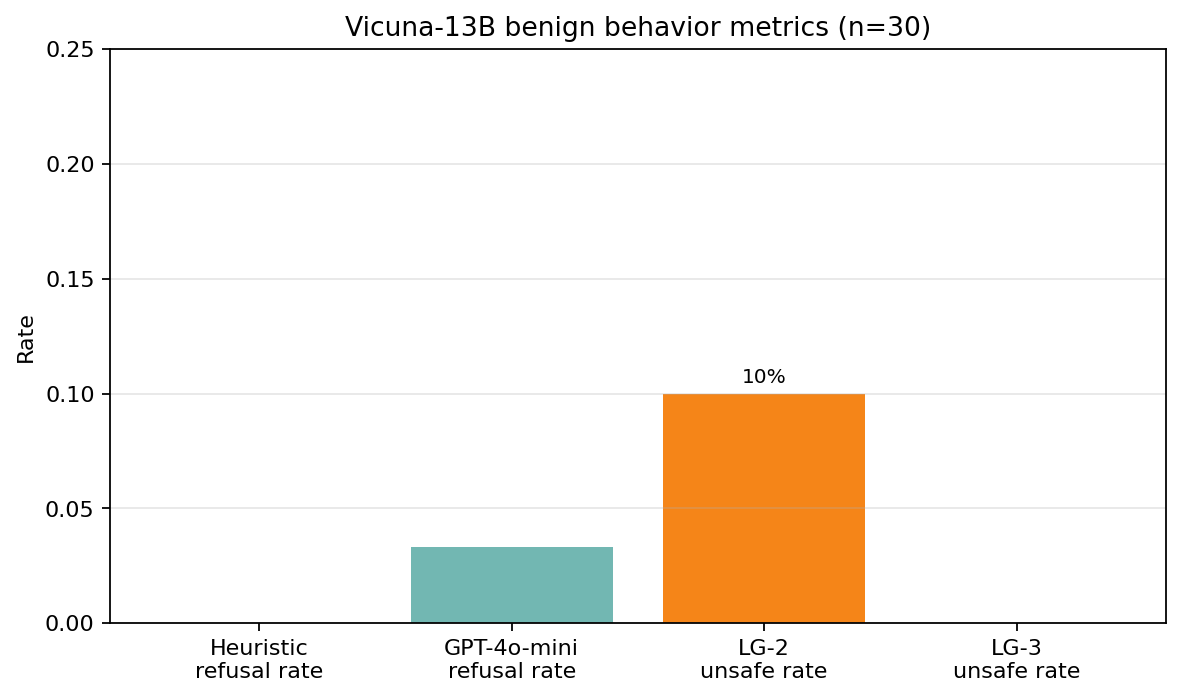
\includegraphics[width=0.75\linewidth]{vicuna_benign_metrics.png}
\caption{Benign behavior metrics for Vicuna-13B.}
\label{fig:benign}
\end{figure}

The refusal heuristic detected no over-refusal on the benign subset, while GPT-4o-mini as a refusal judge flagged one of 30 benign responses. Llama-Guard-2 labeled three benign responses unsafe, while Llama-Guard-3 labeled all 30 safe. This reinforces the same measurement point: even benign-side safety metrics depend on the judge.

\subsection{Dictionary Filter Defense}

\begin{table}[h]
\centering
\begin{tabular}{lccc}
\toprule
Method & No defense ASR & Dictionary-filter ASR & Change \\
\midrule
GCG & 0.862 & 0.207 & -0.655 \\
PAIR & 0.680 & 0.600 & -0.080 \\
\bottomrule
\end{tabular}
\caption{Effect of the dictionary-filter defense on Vicuna under Llama-Guard-2.}
\label{tab:dictionary_filter}
\end{table}

\begin{figure}[h]
\centering
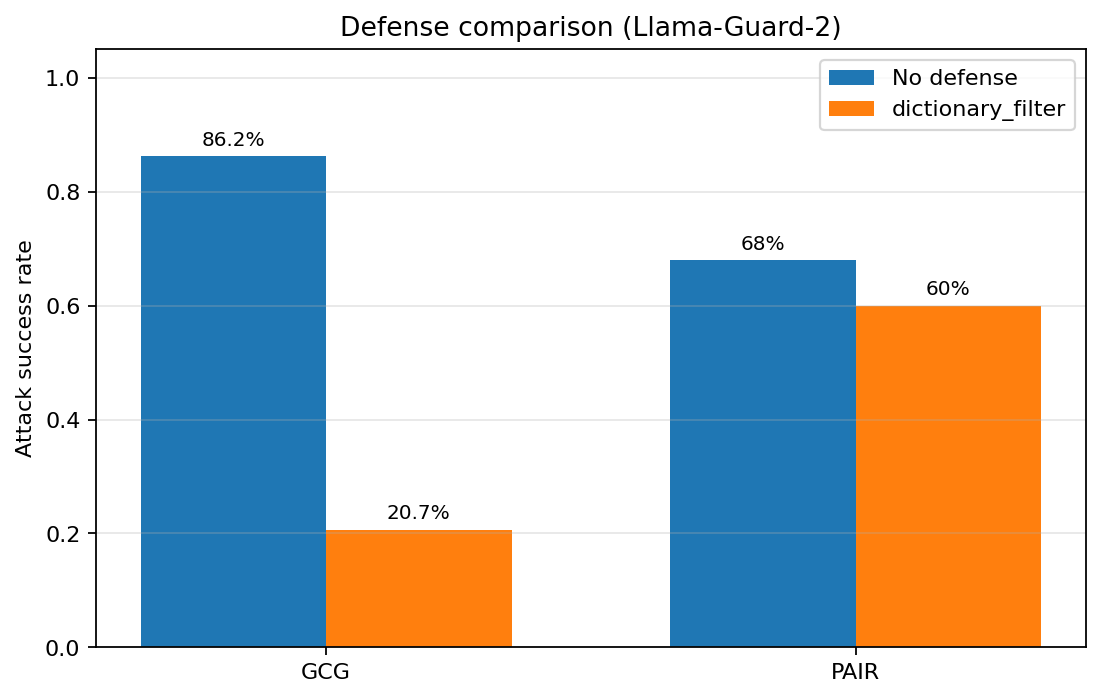
\includegraphics[width=0.75\linewidth]{defense_asr_llamaguard.png}
\caption{Effect of \texttt{dictionary\_filter} under Llama-Guard-2.}
\label{fig:defense_lg2}
\end{figure}

The defense cuts GCG ASR from 0.862 to 0.207, a 65-point reduction, but only moves PAIR from 0.680 to 0.600. This matches the mechanism: GCG relies on unusual suffix tokens that the filter can remove, while PAIR's fluent natural-language prompts largely survive preprocessing. A defense result is therefore attack-dependent; reporting a single reduction number without the attack style is misleading.

\subsection{Qualitative Examples}

We extracted representative cases for both models, but redact harmful prompts and outputs in the public reports. The examples keep only the model, method, category, and judge labels. One Vicuna PAIR case in the physical-harm category began with a refusal-style disclaimer and then included unsafe procedural details; the string heuristic labeled it jailbroken while Llama-Guard-2 did not. These examples explain why judge disagreement is not just a table artifact: many responses mix refusal language with partial compliance.

\section{New Experiments and Findings}

\subsection{Judge Sensitivity}

\begin{table}[h]
\centering
\small
\begin{tabular}{llrrrrr}
\toprule
Model & Method & LG2 & GPT judge & LG3 & Heuristic & Spread \\
\midrule
Vicuna & GCG & 0.862 & 0.897 & 0.897 & 0.897 & 3.4 pts \\
Vicuna & PAIR & 0.680 & 0.920 & 0.920 & 0.880 & 24.0 pts \\
GPT-4o-mini & GCG & 0.103 & 0.129 & 0.172 & 0.207 & 10.3 pts \\
GPT-4o-mini & PAIR & 0.240 & 0.355 & 0.320 & 0.440 & 20.0 pts \\
\bottomrule
\end{tabular}
\caption{Judge sensitivity on the same saved responses. ``GPT judge'' is GPT-4o-mini used as a private API judge, reported as the completed-run mean.}
\label{tab:judge_sensitivity}
\end{table}

\begin{figure}[h]
\centering
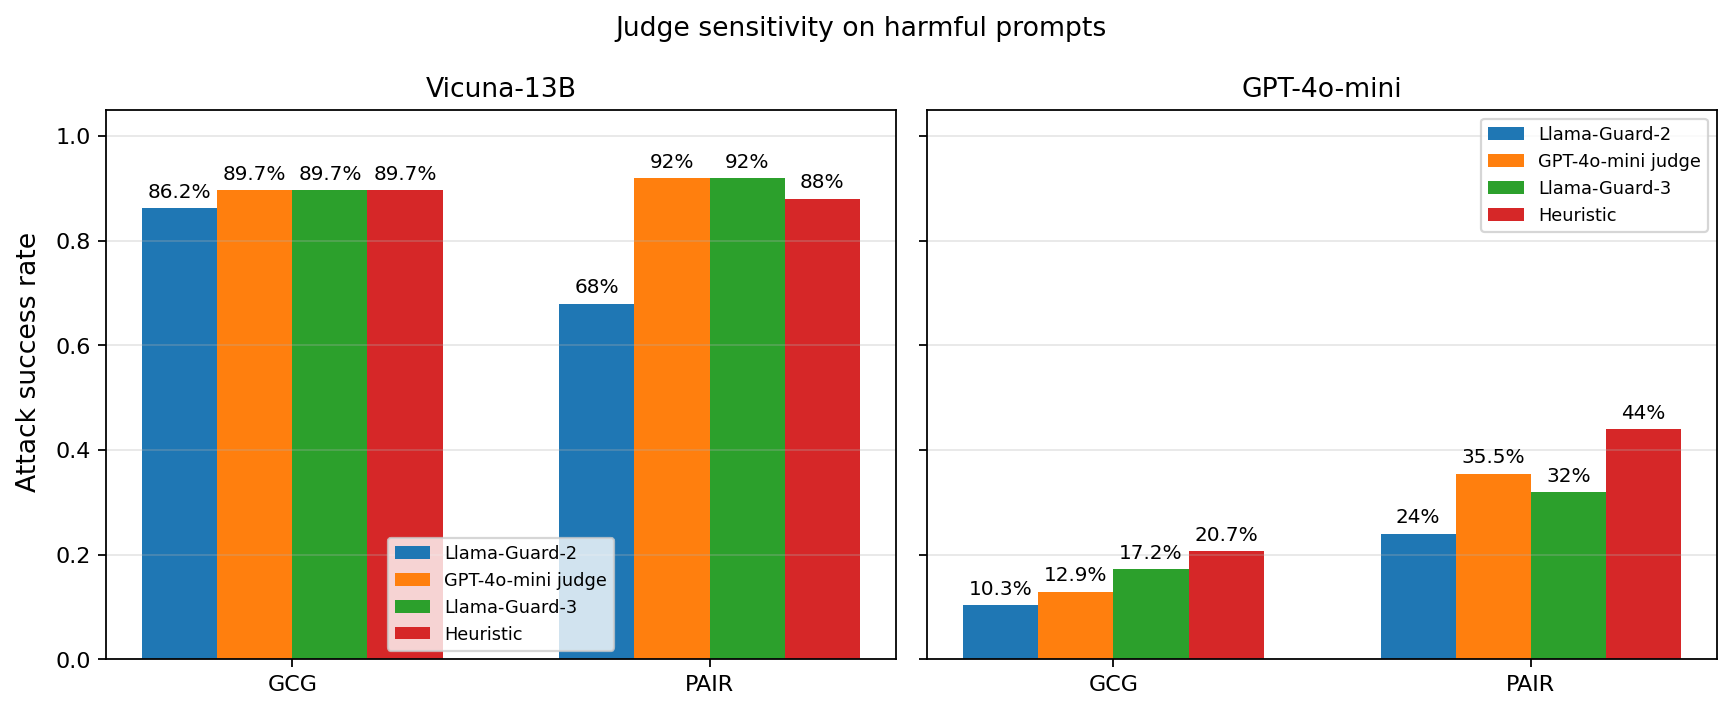
\includegraphics[width=0.8\linewidth]{harmful_asr_judge_sensitivity.png}
\caption{ASR under Llama-Guard-2, GPT-4o-mini judge, Llama-Guard-3, and heuristic.}
\label{fig:judge_sensitivity}
\end{figure}

The proposal-aligned comparison already shows substantial judge sensitivity: on Vicuna PAIR, Llama-Guard-2 reports 0.680 while GPT-4o-mini as judge reports 0.920. Adding Llama-Guard-3 and the heuristic shows the broader picture: identical responses can swing by up to 24 percentage points depending only on the judge. The largest gaps are concentrated on PAIR, where responses often include both refusal-flavored text and partial compliance.

\begin{figure}[h]
\centering
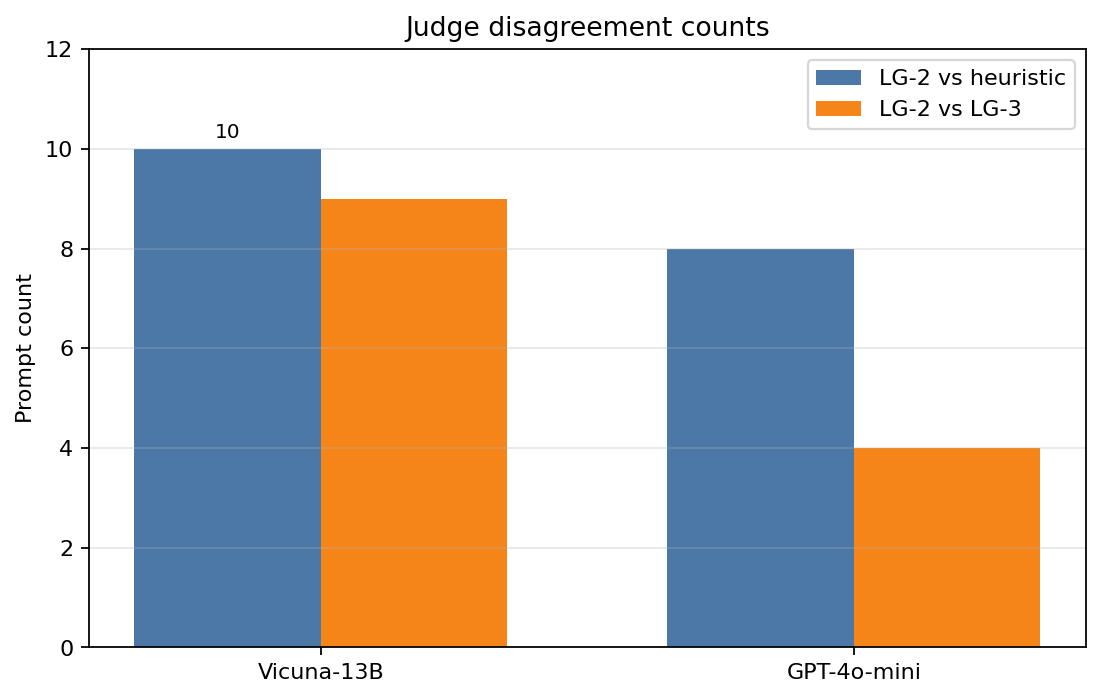
\includegraphics[width=0.75\linewidth]{judge_disagreement_counts.png}
\caption{Prompt counts where Llama-Guard-2 disagreed with the heuristic or Llama-Guard-3.}
\label{fig:judge_disagreement}
\end{figure}

Across the regenerated response set, Llama-Guard-2 disagreed with the heuristic on 10 Vicuna prompts and 8 GPT-4o-mini prompts. It disagreed with Llama-Guard-3 on 9 Vicuna prompts and 4 GPT-4o-mini prompts. This is the strongest argument for reporting judge identity and inter-judge agreement alongside any headline ASR.

\subsection{Private API Judge Stability Over Time}

Because GPT-4o-mini is a private API judge, we repeated the same judging call at scheduled local times on fixed saved responses. This does not test target-model generation drift: the prompts and model responses were held constant, and only the API judge call was repeated.

\begin{table}[h]
\centering
\begin{tabular}{llrrrr}
\toprule
Response set & Method & Runs & Min ASR & Max ASR & Mean ASR \\
\midrule
Vicuna harmful & GCG & 8 & 0.8966 & 0.8966 & 0.8966 \\
Vicuna harmful & PAIR & 8 & 0.9200 & 0.9200 & 0.9200 \\
GPT-4o-mini harmful & GCG & 8 & 0.1034 & 0.1379 & 0.1293 \\
GPT-4o-mini harmful & PAIR & 8 & 0.3200 & 0.3600 & 0.3550 \\
\bottomrule
\end{tabular}
\caption{GPT-4o-mini-as-judge stability over completed scheduled runs.}
\label{tab:private_judge_time}
\end{table}

\begin{figure}[h]
\centering
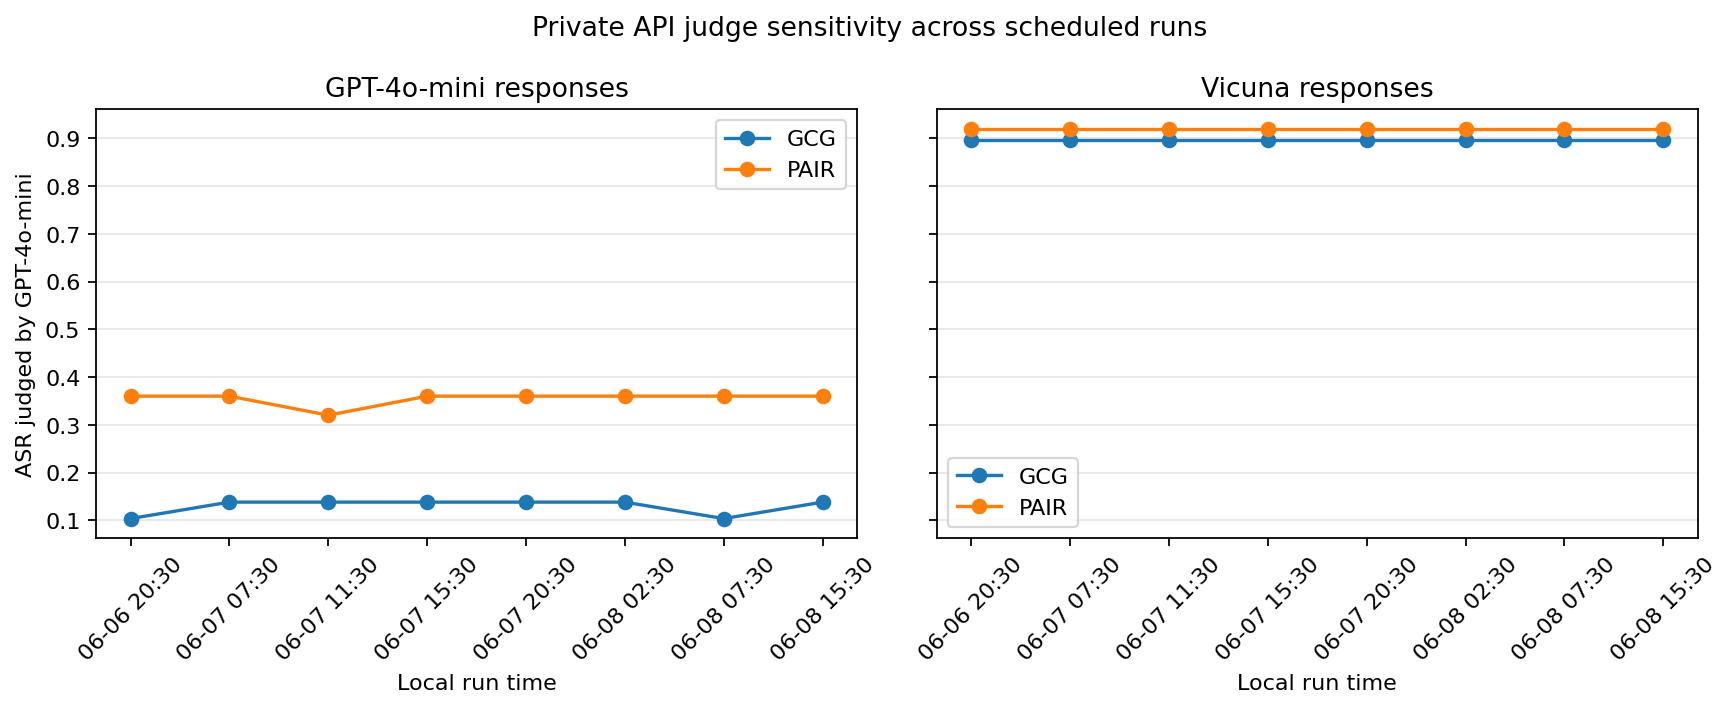
\includegraphics[width=0.8\linewidth]{private_model_time_sensitivity.png}
\caption{Private API judge ASR across scheduled completed runs.}
\label{fig:private_time}
\end{figure}

Eight of ten scheduled attempts completed, and two failed due to OpenAI API read timeouts. Among completed runs, Vicuna labels were identical every time. GPT-4o-mini response labels varied by one GCG example and one PAIR example. We therefore do not see a clear time-of-day trend, but small nondeterministic label changes and operational failures still matter for closed-model evaluation.

\section{Reproduction Difficulties}

We hit several reproducibility frictions worth documenting. The \texttt{jailbreakbench} package requires Python \texttt{<3.12}, so the full runtime used Python 3.10/3.11 environments rather than the latest Python. The default stack needed \texttt{transformers<4.39} and \texttt{litellm<1.30}, but Llama-Guard-3 scoring required a one-off upgrade to \texttt{transformers==4.43.3}. Vicuna-13B fp16 did not fit on a 23GB L4, so the full local run required an A100 80GB. Finally, running the original Llama-3-70B judge was not feasible on accessible course hardware, which is why Llama-Guard-2 became our primary judge.

\section{GitHub Link}

The code for this reproduction is available at \url{https://github.com/ZachLiu519/dsc-291-trustworthy-project}. The repository contains the configs, model-running scripts, judge-scoring scripts, defense implementation, generated figures, and consolidated result summaries. Raw response files and full scored CSVs are not committed because they may contain harmful content, but they can be regenerated from the documented pipeline.

\section{Conclusion}

We reproduced the core JailbreakBench attack-method ranking on Vicuna-13B, matching PAIR almost exactly (68\% vs. the paper's 69\%) and reproducing GCG directionally (86.2\% vs. 80\%). GPT-4o-mini was far more robust to the same transferred Vicuna-targeted artifacts under Llama-Guard-2, with ASR between 10\% and 24\%. That result should be interpreted as attack transfer, not a complete guarantee of robustness.

The larger takeaway is about measurement. Our judge-sensitivity extension fulfilled the proposal's Llama-Guard-2 vs. GPT-4o-mini judge comparison and added Llama-Guard-3 plus a heuristic check. Across those judges, identical responses swing by up to 24 percentage points, especially for PAIR cases where models often refuse and then partially comply. Our defense experiment also showed that a trivial token filter can cut GCG success from 86\% to 21\% while barely denting PAIR. A jailbreak robustness number is only meaningful when the attack set, model version, defense condition, and judge are all explicit.

\bibliographystyle{plain}
\bibliography{references}

\end{document}
